\documentclass[conference]{IEEEtran}


\usepackage[utf8]{inputenc}
\usepackage{graphicx}
\usepackage{listings}
\usepackage{hyperref}

\hyphenation{op-tical net-works semi-conduc-tor}


\begin{document}

\title{Introducción al Análisis de Textos}
% author names and affiliations
\author{\IEEEauthorblockN{Cristobal Donoso Oliva}
\IEEEauthorblockA{Dpto. Ciencias de la Computación\\Facultad de Ingeniería\\
Universidad de Concepción\\
Email: cridonoso@udec.cl}
\and
\IEEEauthorblockN{Rosa Figueroa, Christopher Flores}
\IEEEauthorblockA{Ing. Civil Biomédica\\
Facultad de Ingeniería\\Universidad de Concepción\\
Email: rosa.figueroa@biomedica.udec.cl, chrisflores@udec.cl}
}

% make the title area
\maketitle
% As a general rule, do not put math, special symbols or citations
% in the abstract
\begin{abstract}
El texto plano es difícil de procesar automáticamente puesto que una maquina carece de conocimiento experto y sentido común. Para ello, técnicas como estandarización o limpieza sobre el contenido son fundamentales para extraer información. En el presente informe se muestra una introducción al análisis de textos utilizando herramientas computacionales y lingüísticas.
\end{abstract}
\IEEEpeerreviewmaketitle

\section{Introducción}
El análisis de textos consiste en encontrar y extraer información desde texto plano. Una persona podría realizar este proceso de manera sencilla, sin embargo, la cantidad de documentos (y palabras en éste) a analizar podría significar una gran cantidad de tiempo. Alternativamente, podemos hacer uso de algoritmos especializados en las distintas subdivisiones de la minería de textos (MT) [1].\\\\ MT como área de estudio constituye un gran desafío para los investigadores - pues consiste en una convergencia de distintas áreas de especialidad, que van desde la lingüística a las ciencias de la computación.\\\\En el presente informe se dará una introducción a la minería de textos haciendo uso de la famosa novela \textit{The adventures of Sherlock Holmes} de Conan Doyle [2]. En la \textit{sección 2} se describe el pre-procesamiento realizado antes de trabajar con el texto. La \textit{sección 3} muestra distintas operaciones a realizar con el objetivo de extraer información desde el contenido del libro. Finalmente en la \textit{sección 4} se presentan las conclusiones del trabajo.\\\\{\scriptsize \url{https://github.com/cridonoso/intro_to_text_mining.git}}

\section{Preprocesamiento del texto}
Comúnmente, antes de analizar el texto debemos estandarizar el contenido léxico, así también, es necesario realizar una limpieza de palabras cuyo aporte no es significativo en el proceso.
\subsection{Estandarizando el texto}
Una de las maneras de estandarizar el texto es \textbf{convertir todas las palabras en minúsculas}. No siempre es recomendable realizar ésto, ya que que dependiendo del objetivo (por ejemplo, extraer sustantivos propios o abreviaciones) podemos perder información valiosa. Para efectos de este trabajo el uso de mayúsculas no es significativo.
\subsection{Limpieza del texto}
La limpieza del texto consiste en disminuir la densidad de palabras. Esto con el fin tanto de optimizar la complejidad del algoritmo como de evitar ambigüedades y duplicidad de términos. En particular aplicamos tres operaciones [3]:
\begin{enumerate}
\item \textbf{Tokenización:} Consiste en la división del texto en palabras, frases u otras partes significativas llamadas tokens. En otras palabras se lleva a cabo una segmentación del texto considerando solo caracteres alfanuméricos delimitados por caracteres no alfanuméricos (por ejemplo signos de puntuación, espacios en blanco, entre otros)
\item \textbf{Eliminación de Stopwords:} Las stopwords son palabras cuya dependencia no responde a un tópico en especifico y por lo tanto la información que aportarán es mínima (por ejemplo, conjunciones, artículos, preposiciones, entre otros) 
\item \textbf{Stemming:} El proceso de stemming se trata de encontrar las raíces de la palabras. Una raíz se puede entender como el conjunto mínimo de caracteres desde donde deriva una palabra (Por ejemplo una consulta sobre "bibliotecas" también encuentra documentos en los que solo aparezca "bibliotecario" porque el stem de las dos palabras es el mismo ("bibliotec")).
\end{enumerate}

\section{Extrayendo información desde el texto}
Haciendo uso (parcial o completo) de las técnicas vistas en la sección anterior mostraremos algunas de las aplicaciones.
\subsection{Longitudes}
Una información relevante a la hora de procesar el texto es saber que palabra es la más larga. Así mismo, podmeos encontrar cual tiene más vocales o consonantes. Para ello simplemente tokenizamos el texto en minúscula con el objetivo de limpiar el contenido. Luego seleccionamos las palabras únicas (para no volver a computar el mismo token).

\subsection{Frecuencia de palabras}
Por otro lado, podemos contar las palabras en el texto. Aquí se justifica muy bien la transformación a minúsculas puesto que de otra forma podríamos contar una misma palabra más de una vez. La \textit{figura 1} muestra las 10 palabras con más y menos frecuencia en el texto. Nótese que aparecen términos como puntuaciones y comillas, podemos eliminar estos caracteres con el objetivo de encontrar solo las palabras de interés. La \textit{figura 2} muestra los términos lexicográficos más frecuentes.
\begin{figure}
\begin{center}
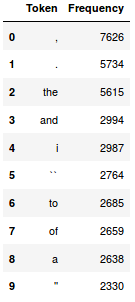
\includegraphics[scale=0.5]{img/1.png}
\hspace{2cm}
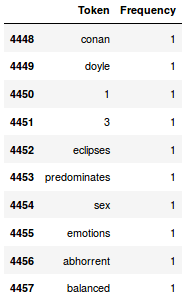
\includegraphics[scale=0.5]{img/2.png} 
\end{center}
\caption{\textbf{[Derecha]} Tabla que reúne los 10 términos con más ocurrencias en el texto. \textbf{[Izquierda]} Tabla que muestra los 10 términos con menos frecuencia en el texto}
\end{figure}

\begin{figure}
\begin{center}
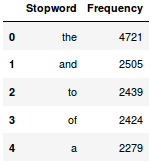
\includegraphics[scale=0.5]{img/3.png}
\end{center}
\caption{Los 5 primeros términos más frecuentes luego de eliminar stopwords.}
\end{figure}
\subsection{Ley de Zipf}
La ley de Zipf [4] tiene diversas aplicaciones [5]. En textos, describe la distribución de las palabras en un corpus en función de su frecuencia. De esta manera se pueden observar empíricamente fenómenos como que la concentración máxima de palabras consiste en la repetición de un pequeño conjunto de términos. La \textit{figura 3} muestra gráficamente la distribución de frecuencias.
\begin{figure}
\begin{center}
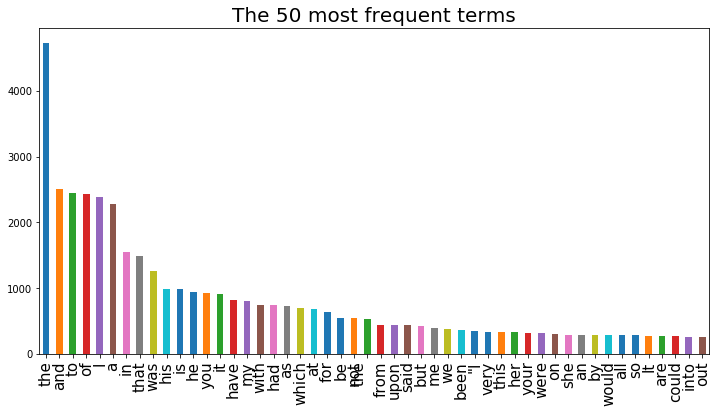
\includegraphics[scale=0.35]{img/4.png} 
\end{center}
\caption{Porción del grafico que muestra el cumpliento de la ley de Zipf en el texto de Sherlock Holmes}
\end{figure}
\subsection{Variación porcentual en la diversidad léxica}
La diversidad léxica varía cuando aplicamos métodos de limpieza como Stemming. Al aplicar esta operación la cantidad de palabras disminuye ya que agrupamos términos utilizando su raíz. Podemos dar cuenta que la variación disminuye al eliminar las stopwords. Esto se debe a la eliminación a priori de palabras que concentran una mayor frecuencia y cuya raíz es el mismo término. Por ejemplo, la raíz de conectores o articulos generalmente son lo mismo.
\begin{center}
\begin{tabular}{|c|c|}
\hline 
\textbf{raiz} & \textbf{palabra} \\ 
\hline 
other & other \\ 
\hline 
same & same \\ 
\hline 
and & and \\ 
\hline 
our & our \\ 
\hline 
it & it \\ 
\hline 
\end{tabular} 
\end{center}
\section{Discusión y Conclusión}
Hemos revisado algunas técnicas y operaciones que comúnmente se utilizan al realizar análisis de textos. Es importante mencionar que la aplicación de cada una de las operaciones varía según el objetivo de la investigación y el tipo de información a extraer.\\\\El trabajo mostró una breve introducción en el procesamiento automático de textos, sin embargo, ésto constituye un buen comienzo para luego utilizar algoritmos de clasificación o clustering. De esta forma, entrenar modelos de aprendizaje - cuyos resultados permiten detectar patrones en el contenido de documentos - genera grandes avances en el descubrimiento de nuevo conocimiento.\\\\Finalmente, quedan pendientes métodos más sofisticados para extraer información semántica o apegadas al contexto (como una ironía o sentimientos [6]). Aún así, el pre-procesamiento es fundamental en toda aplicación que vincule la minería de textos.  
\begin{thebibliography}{1}

\bibitem{IEEEhowto:kopka}
Allahyari, M., Pouriyeh, S., Assefi, M., Safaei, S., Trippe, E. D., Gutierrez, J. B., \& Kochut, K. (2017). A brief survey of text mining: Classification, clustering and extraction techniques. arXiv preprint arXiv:1707.02919.

\bibitem{IEEEhowto:kopka}
Book, V. B. (1981). The Adventures of Sherlock Holmes. \\Plain text: https://sherlock-holm.es/stories/plain-text/advs.txt

\bibitem{IEEEhowto:kopka}
Uysal, A. K., \& Gunal, S. (2014). The impact of preprocessing on text classification. Information Processing \& Management, 50(1), 104-112.

\bibitem{IEEEhowto:kopka}
Li, W. (1992). Random texts exhibit Zipf's-law-like word frequency distribution. IEEE Transactions on information theory, 38(6), 1842-1845.

\bibitem{IEEEhowto:kopka}
Gabaix, X. (1999). Zipf's law for cities: an explanation. The Quarterly journal of economics, 114(3), 739-767.

\bibitem{IEEEhowto:kopka}
Tang, D., Qin, B., \& Liu, T. (2015). Document modeling with gated recurrent neural network for sentiment classification. In Proceedings of the 2015 conference on empirical methods in natural language processing (pp. 1422-1432).
\end{thebibliography}




% that's all folks
\end{document}


